\PassOptionsToPackage{table}{xcolor}

\documentclass[oneside]{ausarbeitung}

\bibliography{bibliography}

\usepackage{tikz}
\usepackage{listings}
\lstset{numbers=left, numberstyle=\tiny, numbersep=5pt}
\lstset{language=C}
\lstset{ % ... whatever was already there ...
        literate=% ... any other literates already there ...
                 {!}{!}1
                 {?}{?}1
                 {:}{:}1
}

\usepackage{xcolor}

\definecolor{lightblue}{RGB}{117, 200, 255}
\definecolor{lightgreen}{RGB}{84, 255, 129}

\colorlet{punct}{red!60!black}
\definecolor{background}{HTML}{EEEEEE}
\definecolor{delim}{RGB}{20,105,176}
\colorlet{numb}{magenta!60!black}

\lstdefinelanguage{json}{
    basicstyle=\normalfont\ttfamily,
    numbers=left,
    numberstyle=\scriptsize,
    stepnumber=1,
    numbersep=8pt,
    showstringspaces=false,
    breaklines=true,
    literate=
     *{0}{{{\color{numb}0}}}{1}
      {1}{{{\color{numb}1}}}{1}
      {2}{{{\color{numb}2}}}{1}
      {3}{{{\color{numb}3}}}{1}
      {4}{{{\color{numb}4}}}{1}
      {5}{{{\color{numb}5}}}{1}
      {6}{{{\color{numb}6}}}{1}
      {7}{{{\color{numb}7}}}{1}
      {8}{{{\color{numb}8}}}{1}
      {9}{{{\color{numb}9}}}{1}
      {:}{{{\color{punct}{:}}}}{1}
      {,}{{{\color{punct}{,}}}}{1}
      {\{}{{{\color{delim}{\{}}}}{1}
      {\}}{{{\color{delim}{\}}}}}{1}
      {[}{{{\color{delim}{[}}}}{1}
      {]}{{{\color{delim}{]}}}}{1},
}

\newcommand*{\captionsource}[2]{%
  \caption[{#1}]{%
    #1%
    \\\hspace{\linewidth}%
    \textbf{Quelle:} #2%
  }%
}

\newcommand*{\quotize}[1]{\glqq #1\grqq}


% ----------------------------------------------------------------------

\begin{document}

\selectlanguage{ngerman}

%--- Art der Arbeit
% Erlaubte Werte:
% Praxissemesterbericht, Projektbericht, Bachelorarbeit oder                                % Masterarbeit
\doctype{Bachelorarbeit}

%--- Studiengang:
\depname{Medieninformatik}

\title{WebGPU}

\author{Laurin Agostini}
\matrikelnr{60526}

\examinerA{Prof.~Dr.~Winfried~Bantel}
\date{XX. Juni 2020}

%--- Titelseite Anzeigen
\maketitle
\cleardoublepage

%---
\pagenumbering{roman}
\setcounter{page}{1}


%--- Eidesstattliche Erklärung anzeigen
\makeaffirmation
\cleardoublepage

%---
\chapter*{Kurzfassung}
\addcontentsline{toc}{chapter}{Kurzfassung}
In dieser Bachelorarbeit geht es um die neuartige Grafik-API WebGPU, die einen Nachfolger zu WebGL darstellt. Mit WebGPU ist es möglich, detaillierte 3D-Szenen, aufwendige Simulationen und XXX in Echtzeit direkt im Webbrowser zu berechnen und darzustellen. 

%-----------------------------------------------------------------------
\cleardoublepage
\addcontentsline{toc}{chapter}{Inhaltsverzeichnis}
\tableofcontents

%---
\addcontentsline{toc}{chapter}{Abbildungsverzeichnis}
\listoffigures

%---
\addcontentsline{toc}{chapter}{Tabellenverzeichnis}
\listoftables

%---
\chapter*{Abkürzungsverzeichnis}
\addcontentsline{toc}{chapter}{Abkürzungsverzeichnis}
\begin{acronym}[JSON]  % Längstes Kürzel in der nachfolgenden
                       % Liste um die Breite der Spalte für die
                       % Abkürzungen zu bestimmen.

%% Eintrag: \acro{Referenzname}[Kürzel]{Langform}
%% Im Text wird die Abkürzung dann mit \ac{Referenzname} benutzt.
\acro{json}[JSON]{JavaScript Object Notation}
\acro{CPU}[CPU]{Central Processing Unit (dt. Hauptprozessor)}
\acro{GPU}[GPU]{Graphics Processing Unit (dt. Grafikprozessor)}
\acro{SMT}[SMT]{Simultaneous Multithreading}
\acro{PCIe}[PCIe]{Peripheral Component Interconnect Express}
\acro{API}[API]{Application Programming Interface (dt. Programmierschnittstelle)}
\end{acronym}
%---
\cleardoublepage
\pagenumbering{arabic}
\setcounter{page}{1}

% ----------------------------------------------------------------------
\chapter{Einleitung}
\label{cha:einleitung}

\section{Motivation}
\label{sec:motivation}

\section{Problemstellung und -abgrenzung}
\label{sec:problemstellung}

\section{Ziel der Arbeit}
\label{sec:ziel}

\section{Vorgehen}
\label{sec:vorgehen}


% ---
\chapter{Grundlagen}
\label{cha:grundlagen}

\section{GPU}
\label{sec:GPU}

\subsection{Aufgaben und Unterschied zur CPU}
\label{sub:GPU_tasks}
Wie der Name, \textit{\textbf{Grafik}prozessor} oder \textit{\textbf{graphics} processing unit}, schon andeutet, ist der Primärzweck einer \ac{GPU} die Erstellung und Manipulation von Bildinhalten und anschließender Ausgabe dieser an ein Anzeigegerät. Während eine \ac{CPU} generell darauf ausgelegt ist, ein weites Spektrum von Aufgaben möglichst schnell nacheinander abzuarbeiten, ist eine \ac{GPU} darauf spezialisiert möglichst viele einfache Aufgaben parallel abzuarbeiten. Diesen Unterschied sieht man direkt, wenn man die Leistungsdaten aktueller \ac{CPU}s und \ac{GPU}s vergleicht:

\begin{minipage}{1.0\textwidth}
\begin{center}
\begin{tabular}{ |l|r|r|r| }
    \hline
    Name & Anzahl Kerne & Basis-/Turbotakt (MHz) & Erscheinungsjahr \\
    \hline
    \multicolumn{4}{|c|}{High-end} \\
    \hline
    \rowcolor{lightblue}
    Intel® Core™ i9-9900K \cite{intel:i9_9900k} & 8 & 3.600 / 5.000 & 2018 \\
    \rowcolor{lightgreen}
    NVIDIA GeForce RTX 2080Ti \cite{nvidia:rtx_2080ti} & 4.352 & 1.350 / 1.545 & 2018 \\
    \hline
    \multicolumn{4}{|c|}{Low-end} \\
    \hline
    \rowcolor{lightblue}
    Intel® Core™ i3-9100 \cite{intel:i3_9100} & 4 & 3.600 / 4.200 & 2019 \\
    \rowcolor{lightgreen}
    NVIDIA GeForce GTX 1650 \cite{nvidia:gtx_1650} & 896 & 1.485 / 1.665 & 2018 \\
    \hline
\end{tabular}
\end{center}
Legende: \colorbox{lightblue}{\ac{CPU}} \colorbox{lightgreen}{\ac{GPU}}
\end{minipage}

Hier sieht man sofort, dass \ac{GPU}s eine um mehrere Größenordnungen höhere Anzahl von Kernen haben, welche allerdings mit einer niedrigeren Taktrate laufen. Zwar konnte in den letzten Jahren ein starker Anstieg von Prozessorkernen in Endbenutzer-\ac{CPU}s beobachtet werden, doch auch eine explizite Workstation-\ac{CPU}, wie ein AMD Ryzen™ Threadripper™ 3990X \cite{amd:threadripper_3990x} mit 64 physischen und durch \ac{SMT} 128 logischen Prozessorkernen ist weit von den Kernzahlen einer aktuellen Einstiegs-\ac{GPU} entfernt. Wie schon angemerkt, kann man die Prozessorkerne von \ac{CPU}s und \ac{GPU}s nicht direkt vergleichen, jedoch zeigen sie deutlich die Spezialisierung der \ac{GPU}s auf parallele Verarbeitung mit einem erhöhtem Datendurchsatz.
Zu den typischen Aufgaben einer \ac{GPU} gehören heutzutage Grafik-, Rechen-, Medien- und Displayfunktionalitäten. 

\subsection{Integrierte und dedizierte GPUs}
\label{sub:GPU_dedicated_integrated}
Mittlerweile haben die meisten Endbenutzer-\ac{CPU}s eine integrierte \ac{GPU} (oft auch \textbf{iGPU} genannt) um die üblichen Multimediaaufgaben zu beschleunigen und Last von der \ac{CPU} zu nehmen. Integrierte \ac{GPU}s sind aber für aufwendige Berechnungen wie zum Beispiel für grafikintensive Anwendungen nicht ausreichend. Dafür werden dedizierte Grafikkarten benötigt, welche der \ac{GPU} dedizierten (daher der Name) Arbeitsspeicher und oft auch eine aktive Kühlung bereitstellen. Grafikkarten werden heutzutage meist über \ac{PCIe} angeschlossen.

\begin{figure}
    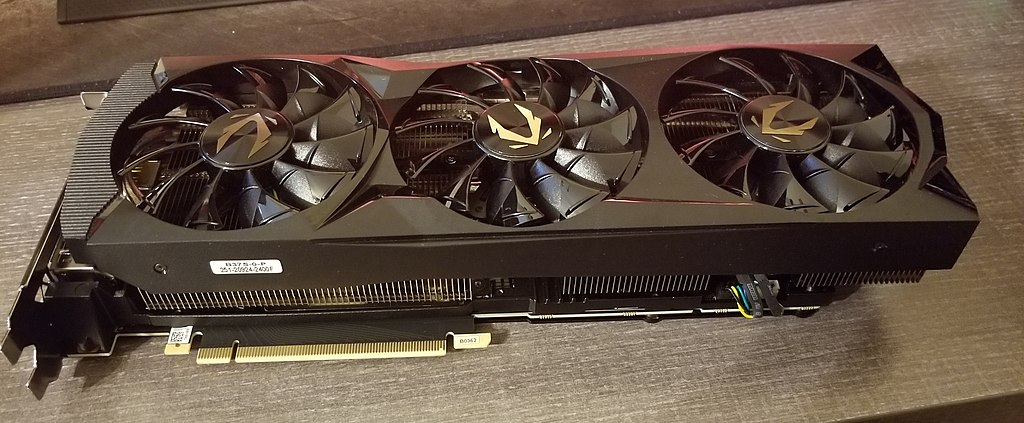
\includegraphics[width=\textwidth]{images/1024px-Zotac_Gaming_GTX_2080_ti.jpg}
    \caption{Beispiel einer Grafikkarte (Zotax Gaming 2080 ti) \cite{2080_ti_graphics_card}}
    \label{fig:2080_ti_graphics_card}
\end{figure}

\subsection{Geschichte \cite[Vgl.][]{gpu_history}}
\label{sub:GPU_history}
\textit{Der Begriff \quotize{\ac{GPU}} wurde erst 1999 von NVIDIA eingeführt, jedoch werden im folgenden der Einfachheit halber alle vorherigen Prozessoren mit ähnlicher Funktion unter dem Begriff \quotize{\ac{GPU}} zusammengefasst.}

Bis in die frühen 1980er Jahre waren \ac{GPU}s nicht mehr als integrierte Bildspeicher und dafür zuständig einfache Linienformen auf den Rasterbildschirm zu zeichnen. Erst ab 1987 wurden weitere Funktionen hinzugefügt. So zum Beispiel Rasterisierung von Polygonenflächen (anstatt von Polygonkanten), Vertex Beleuchtung, Tiefenpuffer und Farbüberblendung. Im Jahre 1992 wurde von Silicon Graphics Inc. mit OpenGL, die bis heute meist verwendete und unterstützte \ac{API} für Grafikprogrammierung eingeführt.

%---
\chapter{Problemanalyse}
\label{cha:problemanalyse}


%---
\chapter{Implementierung}
\label{cha:implementierung}



%---
\chapter{Evaluierung}
\label{cha:evaluation}


%---
\chapter{Zusammenfassung und Ausblick}
\label{cha:zusammenfassung}
\section{Erreichte Ergebnisse}
\label{sec:ergebnisse}


\section{Ausblick}
\label{sec:ausblick}

\subsection{Erweiterbarkeit der Ergebnisse}
\label{sub:erweiterbarkeit}

\subsection{Übertragbarkeit der Ergebnisse}
\label{sub:uebertragbarkeit}

%-----------------------------------------------------------------------
\appendix

%---
\addcontentsline{toc}{chapter}{Referenzen}
\printbibliography[title={Referenzen}]

%---
%\chapter{Anhang A}

%---
%\chapter{Anhang B}


\end{document}